\documentclass[a4paper, 12pt, italian]{report}
\usepackage{ctable}
\usepackage{url}
\usepackage[utf8]{inputenc}
\usepackage{enumitem}
\usepackage{graphicx}
\usepackage{longtable}
\usepackage{amsmath}
\usepackage[italian]{babel}
\usepackage{color}
\usepackage{listings}

\usepackage[raggedright]{titlesec}
\usepackage{blindtext}

\titleformat{\chapter}[hang]{\bfseries\huge}{\thechapter.}{2pc}{}
\titlelabel{\thetitle.\quad}   % For consistency in all headings

 \definecolor{Gray}{gray}{0.8}
\newcolumntype{a}{>{\columncolor{Gray}}p{.25\textwidth}}

\begin{document}

% === Per gli snippet =====================================
\definecolor{mygreen}{rgb}{0,0.6,0}
\definecolor{mygray}{rgb}{0.5,0.5,0.5}
\definecolor{mymauve}{rgb}{0.58,0,0.82}
\lstset{
backgroundcolor=\color{white}, % choose the background color; you must add \usepackage{color} or \usepackage{xcolor}
basicstyle=\footnotesize\ttfamily, % the size of the fonts that are used for the code
breakatwhitespace=false, % sets if automatic breaks should only happen at whitespace
breaklines=true, % sets automatic line breaking
captionpos=n, % sets the caption-position to bottom
commentstyle=\color{mygreen}, % comment style
deletekeywords={}, % if you want to delete keywords from the given language
escapeinside={\%}{)}, % if you want to add LaTeX within your code
extendedchars=false, % lets you use non-ASCII characters; for 8-bits encodings only, does not work with UTF-8
frame=single, % adds a frame around the code
keepspaces=true, % keeps spaces in text, useful for keeping indentation of code (possibly needs columns=flexible)
keywordstyle=\color{blue}, % keyword style
language=Java, % the language of the code
morekeywords={}, % if you want to add more keywords to the set
numbers=left, % where to put the line-numbers; possible values are (none, left, right)
numbersep=5pt, % how far the line-numbers are from the code
numberstyle=\tiny\color{mygray}, % the style that is used for the line-numbers
rulecolor=\color{black}, % if not set, the frame-color may be changed on line-breaks within not-black text (e.g. comments (green here))
showspaces=false, % show spaces everywhere adding particular underscores; it overrides 'showstringspaces'
showstringspaces=false, % underline spaces within strings only
showtabs=false, % show tabs within strings adding particular underscores
stepnumber=1, % the step between two line-numbers. If it's 1, each line will be numbered
stringstyle=\color{mymauve}, % string literal style
tabsize=2, % sets default tabsize to 2 spaces
title=\lstname % show the filename of files included with \lstinputlisting; also try caption instead of title
literate=
  {á}{{\'a}}1 {é}{{\'e}}1 {í}{{\'i}}1 {ó}{{\'o}}1 {ú}{{\'u}}1
  {Á}{{\'A}}1 {É}{{\'E}}1 {Í}{{\'I}}1 {Ó}{{\'O}}1 {Ú}{{\'U}}1
  {à}{{\`a}}1 {è}{{\`e}}1 {ì}{{\`i}}1 {ò}{{\`o}}1 {ù}{{\`u}}1
  {À}{{\`A}}1 {È}{{\'E}}1 {Ì}{{\`I}}1 {Ò}{{\`O}}1 {Ù}{{\`U}}1
  {ä}{{\"a}}1 {ë}{{\"e}}1 {ï}{{\"i}}1 {ö}{{\"o}}1 {ü}{{\"u}}1
  {Ä}{{\"A}}1 {Ë}{{\"E}}1 {Ï}{{\"I}}1 {Ö}{{\"O}}1 {Ü}{{\"U}}1
  {â}{{\^a}}1 {ê}{{\^e}}1 {î}{{\^i}}1 {ô}{{\^o}}1 {û}{{\^u}}1
  {Â}{{\^A}}1 {Ê}{{\^E}}1 {Î}{{\^I}}1 {Ô}{{\^O}}1 {Û}{{\^U}}1
  {œ}{{\oe}}1 {Œ}{{\OE}}1 {æ}{{\ae}}1 {Æ}{{\AE}}1 {ß}{{\ss}}1
  {ç}{{\c c}}1 {Ç}{{\c C}}1 {ø}{{\o}}1 {å}{{\r a}}1 {Å}{{\r A}}1
  {€}{{\EUR}}1 {£}{{\pounds}}1
}
% === Fine ===================================================

\begin{titlepage}
\newcommand{\HRule}{\rule{\linewidth}{0.5mm}} 
\center 
\textsc{\LARGE Università degli studi di Salerno}\\[1cm] 

\includegraphics[width=3.5cm]{img/logo.jpg} \\[1cm]
\textsc{\large Progetto di Fondamenti di Visione Artificiale}\\[0.5cm]
\textsc{\Large Gruppo 2}\\[0.5cm] 
 \HRule \\[0.4cm]
{ \large \bfseries Modulo di estrazione delle caratteristiche dell'orecchio}\\[0.4cm] 
\HRule \\[1.5cm]

\begin{minipage}{0.4\textwidth}
\begin{flushleft} \large
\emph{Autori:}\\
Matteo \textsc{Merola}\\
Simone \textsc{Scalabrino}\\
Carlo \textsc{Branca}\\
\end{flushleft}
\end{minipage}
~
\begin{minipage}{0.4\textwidth}
\begin{flushright} \large
\emph{Supervisore:} \\
Prof. Michele \textsc{Nappi} \\
Dott.ssa Chiara \textsc{Galdi}
\end{flushright}
\end{minipage}\\[2.5cm]


{\Large Documentazione}\\
Versione 1.0\\[1cm]

{\large 28 maggio 2014} % Date, change the \today to a set date if you want to be precise

\vfill

\end{titlepage}		
    %\input{Revision}
	\setcounter{tocdepth}{1}	
	\tableofcontents
	%\listoffigures
	%\listoftables
	
	\chapter{Scopo}
Il modulo ha lo scopo di estrarre delle features da immagini di orecchio segmentate attraverso l'applicazione di due algoritmi:
\begin{itemize}
	\item SIFT (Scale Invariant Feature Transform)
	\item LBP (Local Binary Pattern)
\end{itemize}
	\chapter{Specifica}
L'applicazione realizzata rispetta la seguente specifica:\\\\
\textbf{Input:}
\begin{itemize}
	\item N (definito nel file di configurazione, es N=4) immagini di orecchio segmentate;
	\item Username;
	\item Punteggio qualità;
	\item Azione: registrazione/riconoscimento/verifica;
\end{itemize}
\textbf{Funzionalità principali:}
\begin{itemize}
	\item Estrazione delle caratteristiche con uno o più algoritmi (definito in un file di configurazione);
	\item Salvataggio degli N vettori delle caratteristiche, con associato lo username, in caso di registrazione;
\end{itemize}
\textbf{Output:}
\begin{itemize}
	\item Uno o più vettori delle caratteristiche (a seconda del numero di algoritmi di feature extraction usati);
	\item Username;
	\item Punteggio qualità;
	\item Azione: registrazione/riconoscimento/verifica;
\end{itemize}
	\chapter{Parametri}
Il modulo restituisce un oggetto di tipo Map$<$String, List$<$List$<$IFeature$>>>$ (ovvero una mappa del tipo ``Nome algoritmo -$>$ Lista''). In particolare, la lista contiene n elementi, dove n è il numero di immagini passate in input e, per ogni immagine i, è presente un'ulteriore lista di feature relative all'immagine i-esima.\\
Ad esempio, se sono passate 2 immagini e sono attivi gli algoritmi SIFT e LBP, il valore di ritorno sarà formato così:\\\\

\begin{lstlisting}
Map(
"SIFT",  List(List<IFeature>, List<IFeature>)
"LBP",   List(List<IFeature>, List<IFeature>)
)
\end{lstlisting}
\vspace{0.4cm}
Se sono passate 3 immagini con il solo algoritmo SIFT attivo:\\
\begin{lstlisting}
Map(
"SIFT",  List(List<IFeature>, List<IFeature>, List<IFeature>)
)
\end{lstlisting}
\vspace{0.8cm}
Ad ogni immagine è associata, dunque, una lista di IFeature (per ogni algoritmo). IFeature è un'interfaccia che descrive una feature generica;\\ l'implementazione cambia in base all'algoritmo. In allegato invio i file sorgenti di IFeature, LBPFeature, SIFTFeature (le ultime due sono implementazioni concrete della prima) e Feature (la classe della libreria per il SIFT che noi incapsuliamo in SIFTFeature).\\
L'algoritmo LBP restituisce, per ogni immagine, una singola IFeature (di tipo LBPFeature) che ha al suo interno, come descrittori (variabile "descriptors"), un array di interi.\\
L'algoritmo SIFT restituisce, per ogni immagine, un numero variabile di IFeature (di tipo SIFTFeature) dipendente dall'immagine.\\
La classe IFeature ha un metodo (getDistance(IFeature)) adibito al calcolo della distanza tra due IFeature: il metodo è già implementato per l'algoritmo SIFT (è definito nella libreria che abbiamo utilizzato) ma non per LBP.\\
Le feature sono serializzate nel database in fase di registrazione.\\
	\chapter{Diagrammi}

\section{Strategy Pattern}
Nella programmazione ad oggetti, lo strategy pattern è uno dei pattern fondamentali, definiti originariamente dalla gang of four.

Lo strategy pattern è uno dei pattern comportamentali. L'obiettivo di questa architettura è isolare un algoritmo all'interno di un oggetto. Il pattern strategy è utile in quelle situazioni dove sia necessario modificare dinamicamente gli algoritmi utilizzati da un'applicazione. Si pensi ad esempio alle possibili visite in una struttura ad albero (visita anticipata, simmetrica, posticipata): mediante il pattern strategy è possibile selezionare a tempo di esecuzione una tra le visite ed eseguirla sull'albero per ottenere il risultato voluto. Il design pattern Iterator si basa proprio su questo.

Questo pattern prevede che gli algoritmi siano intercambiabili tra loro (in base ad una qualche condizione) in modo trasparente al client che ne fa uso. In altre parole: la famiglia di algoritmi che implementa una funzionalità (ad esempio di visita o di ordinamento) esporta sempre la medesima interfaccia, in questo modo il client dell'algoritmo non deve fare nessuna assunzione su quale sia la strategia istanziata in un particolare istante.

Nell'applicazione realizzata abbiamo utilizzato questo design pattern per fornire il supporto all'estensione del sistema per l'aggiunta di nuovi algoritmi per l'estrazione delle caratteristiche.

\begin{figure}[ht]
	\centering
	%width=.5\textwidth
	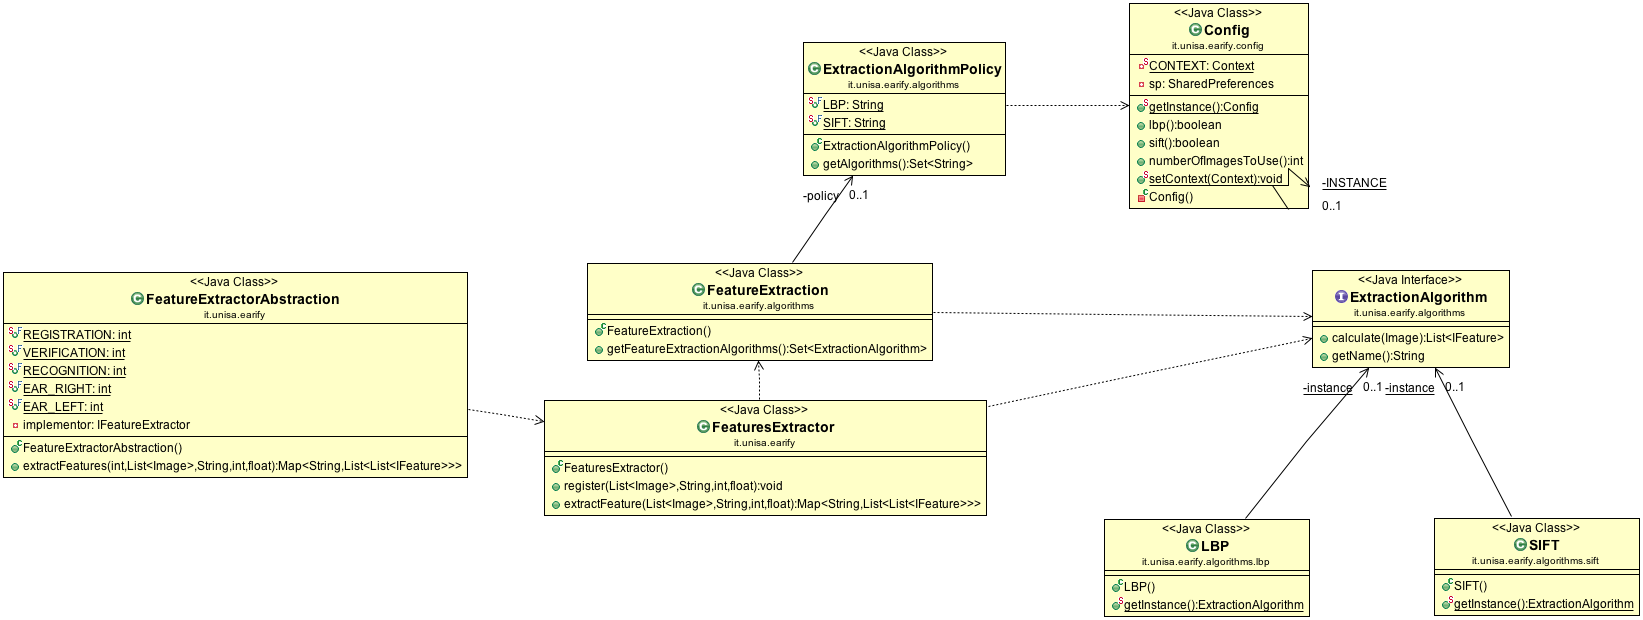
\includegraphics[width=1.5\textwidth, angle=90]{img/strategy.png}
	\caption{Strategy}\label{fig:strategy}
\end{figure}

\section{Bridge Pattern}
Il bridge pattern è un design pattern (modello di progettazione) della programmazione ad oggetti e permette di separare l'interfaccia di una classe (che cosa si può fare con la classe) dalla sua implementazione (come si fa). In tal modo si può usare l'ereditarietà per fare evolvere l'interfaccia o l'implementazione in modo separato.

Abbiamo utilizzato questo design pattern per supportare l'aggiunta di diverse implementazioni del medesimo algoritmo di estrazione. Un esempio di utilizzo di questo pattern può essere individuato nell'implementazione di due versioni dell'algoritmo LBP: una scritta in linguaggio nativo C e l'altra in linguaggio Java.

\begin{figure}[ht]
	\centering
	%width=.5\textwidth
	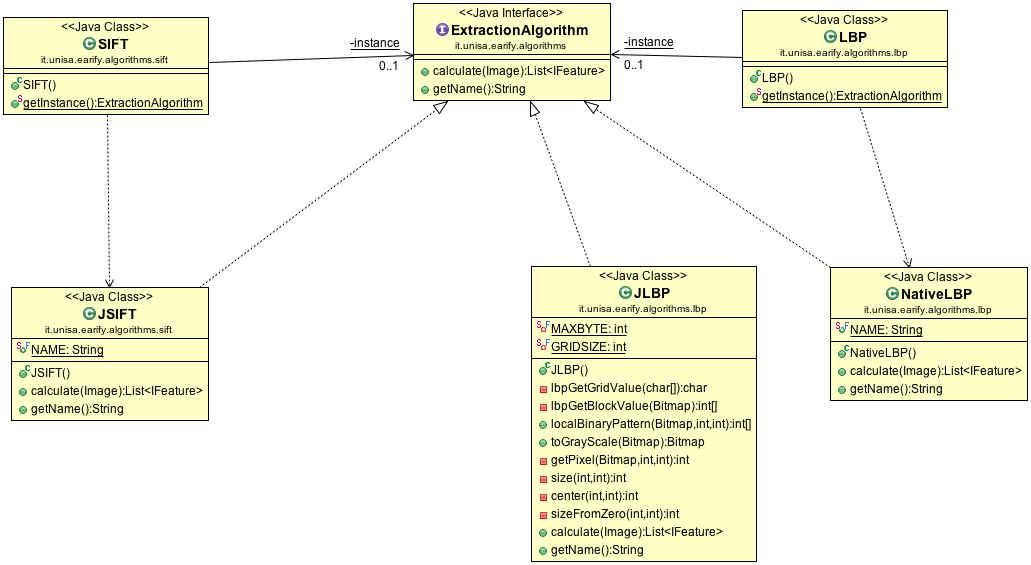
\includegraphics[width=1.5\textwidth, angle=90]{img/bridge.png}
	\caption{Bridge}\label{fig:bridge}
\end{figure}

\section{Observer Pattern}
L'Observer pattern è un design pattern utilizzato per tenere sotto controllo lo stato di diversi oggetti.

È un pattern intuitivamente utilizzato come base architetturale di molti sistemi di gestione di eventi. Molti paradigmi di programmazione legati agli eventi, utilizzati anche quando ancora non era diffusa la programmazione ad oggetti, sono riconducibili a questo pattern. È possibile individuarlo in maniera rudimentale nella programmazione di sistema Windows, o in altri framework di sviluppo che richiedono la gestione di eventi provenienti da diversi oggetti, come ad esempio la funzione "OnMsgProc" per la gestione delle code di messaggi windows.

Sostanzialmente il pattern si basa su uno o più oggetti, chiamati osservatori o listener, che vengono registrati per gestire un evento che potrebbe essere generato dall'oggetto "osservato".

Oltre all'observer esiste il concrete Observer che si differenzia dal primo perché implementa direttamente le azioni da compiere in risposta ad un messaggio; riepilogando il primo è una classe astratta, il secondo no.

Uno degli aspetti fondamentali è che tutto il funzionamento dell'observer si basa su meccanismi di callback, implementabili in diversi modi, o tramite funzioni virtuali o tramite puntatori a funzioni passati quali argomenti nel momento della registrazione dell'observer, e spesso a questa funzione vengono passati dei parametri in fase di generazione dell'evento.

Abbiamo utilizza questo design pattern per fornire un callback alla attività principale dell'applicazione Android al momento in cui il Thread asincrono che effettua l'estrazione tramite gli algoritmi scelti termina la sua esecuzione correttamente o termina a seguito di un'eccezione generata.

\begin{figure}[ht]
	\centering
	%width=.5\textwidth
	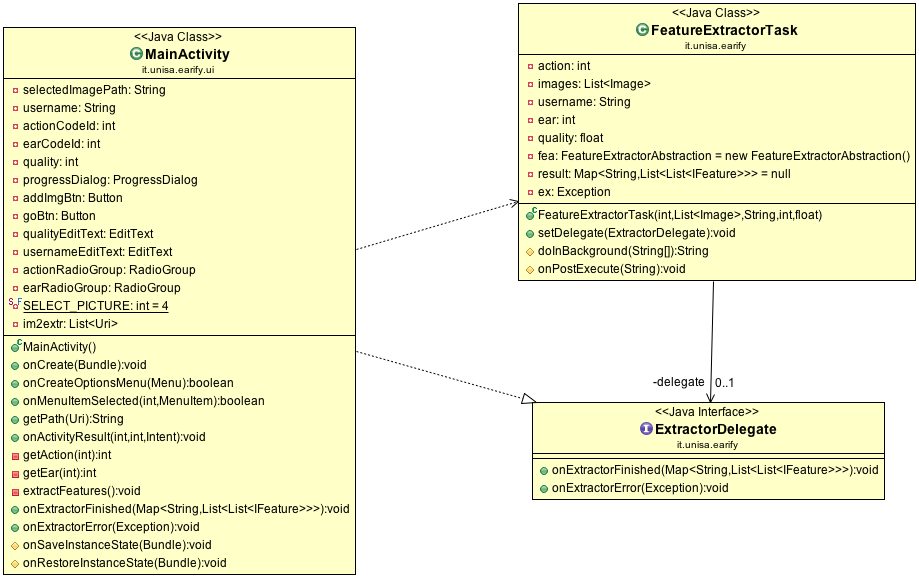
\includegraphics[width=1.5\textwidth, angle=90]{img/delegation.png}
	\caption{Observer}\label{fig:delegation}
\end{figure}

\section{Pacchetti}
L'applicazione si dipana nei pacchetti rappresentati in figura \ref{fig:pkg}.

\begin{figure}[ht]
	\centering
	%width=.5\textwidth
	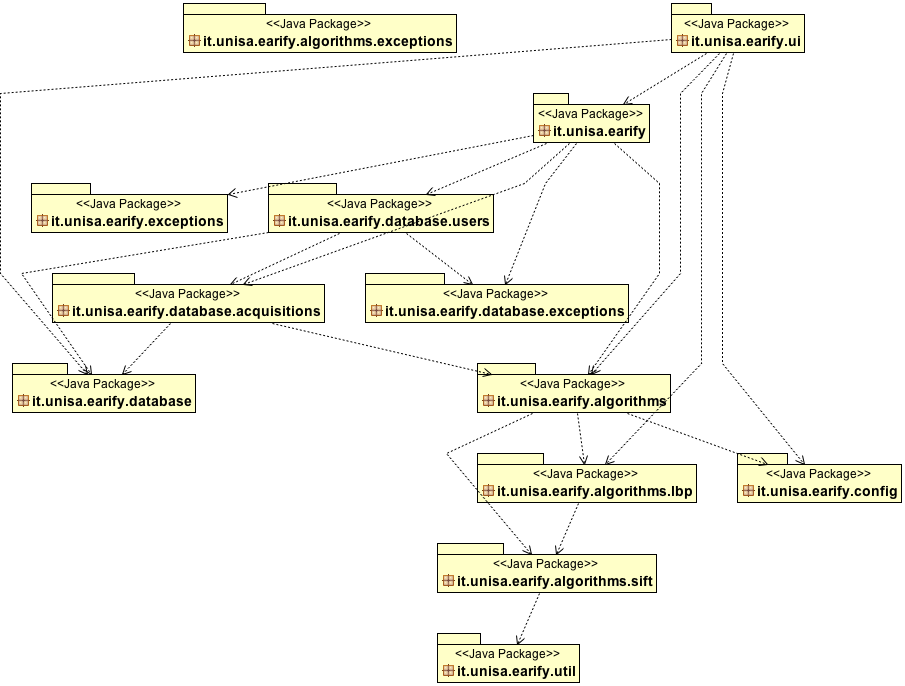
\includegraphics[width=1.5\textwidth, angle=90]{img/pkg.png}
	\caption{Packages}\label{fig:pkg}
\end{figure}

\section{Database}
L'accesso al database embedded nell'applicazione Android avviene tramite le classi diagrammate nella figura \ref{fig:db}.

\begin{figure}[ht]
	\centering
	%width=.5\textwidth
	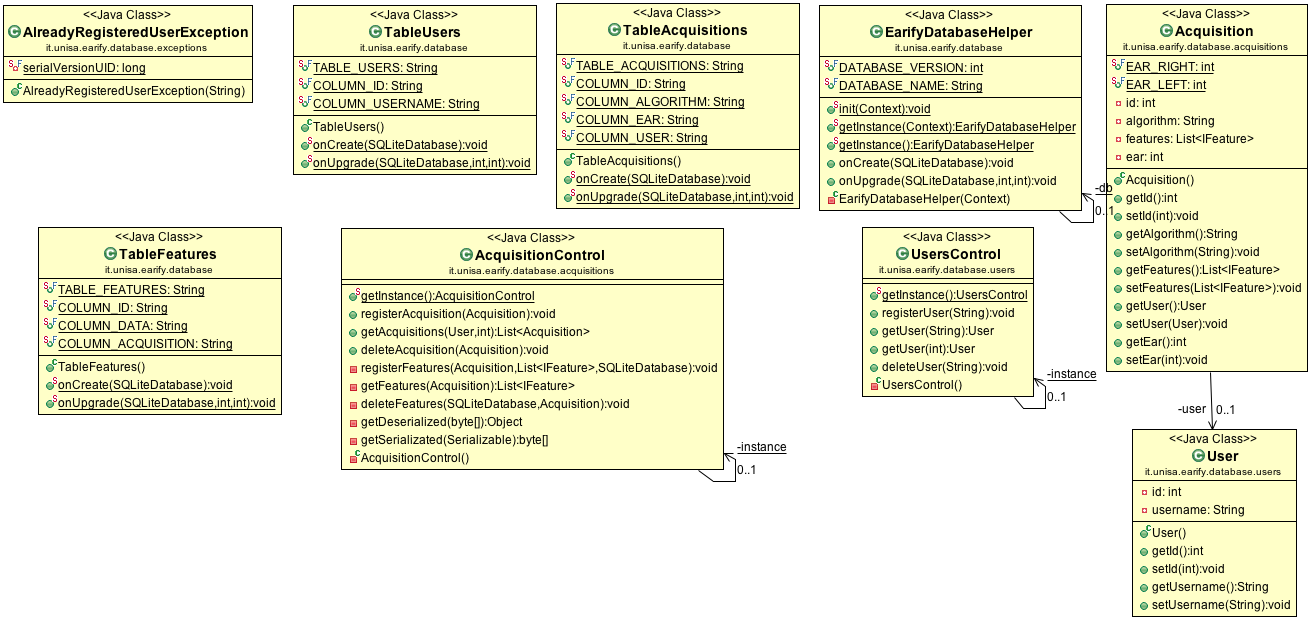
\includegraphics[width=1.5\textwidth, angle=90]{img/db.png}
	\caption{Classi database}\label{fig:db}
\end{figure}


\end{document}
